\documentclass[14pt,russian]{scrartcl}
\let\counterwithout\relax
\let\counterwithin\relax
\usepackage{lmodern}
\usepackage{float}
\usepackage{xcolor}
\usepackage{extsizes}
\usepackage{subfig}
\usepackage[export]{adjustbox}
\usepackage{tocvsec2} % возможность менять учитываемую глубину разделов в оглавлении
\usepackage[subfigure]{tocloft}

\usepackage{fancyvrb}
\usepackage{ulem,bm,mathrsfs,ifsym} %зачеркивания, особо жирный стиль и RSFS начертание
\usepackage{sectsty} % переопределение стилей подразделов
%%%%%%%%%%%%%%%%%%%%%%%

%%% Поля и разметка страницы %%%
\usepackage{pdflscape}                              % Для включения альбомных страниц
\usepackage{geometry}                               % Для последующего задания полей
\geometry{a4paper,tmargin=2cm,bmargin=2cm,lmargin=3cm,rmargin=1cm} % тоже самое, но лучше

%%% Математические пакеты %%%
\usepackage{amsthm,amsfonts,amsmath,amssymb,amscd}  % Математические дополнения от AMS
\usepackage{mathtools}                              % Добавляет окружение multlined
\usepackage[perpage]{footmisc}

%%%% Установки для размера шрифта 14 pt %%%%
%% Формирование переменных и констант для сравнения (один раз для всех подключаемых файлов)%%
%% должно располагаться до вызова пакета fontspec или polyglossia, потому что они сбивают его работу
%\newlength{\curtextsize}
%\newlength{\bigtextsize}
%\setlength{\bigtextsize}{13pt}
\KOMAoptions{fontsize=14pt}

\makeatletter
\def\showfontsize{\f@size{} point}
\makeatother

%\makeatletter
%\show\f@size                                       % неплохо для отслеживания, но вызывает стопорение процесса, если документ компилируется без команды  -interaction=nonstopmode 
%\setlength{\curtextsize}{\f@size pt}
%\makeatother

%шрифт times
\usepackage{tempora}

   %%% Решение проблемы копирования текста в буфер кракозябрами
%    \input glyphtounicode.tex
%    \input glyphtounicode-cmr.tex %from pdfx package
%    \pdfgentounicode=1
    \usepackage{cmap}                               % Улучшенный поиск русских слов в полученном pdf-файле
    \usepackage[T2A]{fontenc}                       % Поддержка русских букв
    \usepackage[utf8]{inputenc}                     % Кодировка utf8
    \usepackage[english, main=russian]{babel}            % Языки: русский, английский
%   \IfFileExists{pscyr.sty}{\usepackage{pscyr}}{}  % Красивые русские шрифты
%\renewcommand{\rmdefault}{ftm}
%%% Оформление абзацев %%%
\usepackage{indentfirst}                            % Красная строка
%\usepackage{eskdpz}

%%% Таблицы %%%
\usepackage{longtable}                              % Длинные таблицы
\usepackage{multirow,makecell,array}                % Улучшенное форматирование таблиц
\usepackage{booktabs}                               % Возможность оформления таблиц в классическом книжном стиле (при правильном использовании не противоречит ГОСТ)

%%% Общее форматирование
\usepackage{soulutf8}                               % Поддержка переносоустойчивых подчёркиваний и зачёркиваний
\usepackage{icomma}                                 % Запятая в десятичных дробях



%%% Изображения %%%
\usepackage{graphicx}                               % Подключаем пакет работы с графикой
\usepackage{wrapfig}

%%% Списки %%%
\usepackage{enumitem}

%%% Подписи %%%
\usepackage{caption}                                % Для управления подписями (рисунков и таблиц) % Может управлять номерами рисунков и таблиц с caption %Иногда может управлять заголовками в списках рисунков и таблиц
%% Использование:
%\begin{table}[h!]\ContinuedFloat - чтобы не переключать счетчик
%\captionsetup{labelformat=continued}% должен стоять до самого caption
%\caption{}
% либо ручками \caption*{Продолжение таблицы~\ref{...}.} :)

%%% Интервалы %%%

%%% Счётчики %%%
\usepackage[figure,table,section]{totalcount}               % Счётчик рисунков и таблиц
\DeclareTotalCounter{lstlisting}
\usepackage{totcount}                               % Пакет создания счётчиков на основе последнего номера подсчитываемого элемента (может требовать дважды компилировать документ)
\usepackage{totpages}                               % Счётчик страниц, совместимый с hyperref (ссылается на номер последней страницы). Желательно ставить последним пакетом в преамбуле

%%% Продвинутое управление групповыми ссылками (пока только формулами) %%%
%% Кодировки и шрифты %%%

%   \newfontfamily{\cyrillicfont}{Times New Roman}
%   \newfontfamily{\cyrillicfonttt}{CMU Typewriter Text}
	%\setmainfont{Times New Roman}
	%\newfontfamily\cyrillicfont{Times New Roman}
	%\setsansfont{Times New Roman}                    %% задаёт шрифт без засечек
%	\setmonofont{Liberation Mono}               %% задаёт моноширинный шрифт
 %   \IfFileExists{pscyr.sty}{\renewcommand{\rmdefault}{ftm}}{}
%%% Интервалы %%%
%linespread-реализация ближе к реализации полуторного интервала в ворде.
%setspace реализация заточена под шрифты 10, 11, 12pt, под остальные кегли хуже, но всё же ближе к типографской классике. 
\linespread{1.3}                    % Полуторный интервал (ГОСТ Р 7.0.11-2011, 5.3.6)
%\renewcommand{\@biblabel}[1]{#1}

%%% Гиперссылки %%%
\usepackage{hyperref}

%%% Выравнивание и переносы %%%
\sloppy                             % Избавляемся от переполнений
\clubpenalty=10000                  % Запрещаем разрыв страницы после первой строки абзаца
\widowpenalty=10000                 % Запрещаем разрыв страницы после последней строки абзаца

\makeatletter % малые заглавные, small caps shape
\let\@@scshape=\scshape
\renewcommand{\scshape}{%
  \ifnum\strcmp{\f@series}{bx}=\z@
    \usefont{T1}{cmr}{bx}{sc}%
  \else
    \ifnum\strcmp{\f@shape}{it}=\z@
      \fontshape{scsl}\selectfont
    \else
      \@@scshape
    \fi
  \fi}
\makeatother

%%% Подписи %%%
%\captionsetup{%
%singlelinecheck=off,                % Многострочные подписи, например у таблиц
%skip=2pt,                           % Вертикальная отбивка между подписью и содержимым рисунка или таблицы определяется ключом
%justification=centering,            % Центрирование подписей, заданных командой \caption
%}
%%%        Подключение пакетов                 %%%
\usepackage{ifthen}                 % добавляет ifthenelse
%%% Инициализирование переменных, не трогать!  %%%
\newcounter{intvl}
\newcounter{otstup}
\newcounter{contnumeq}
\newcounter{contnumfig}
\newcounter{contnumtab}
\newcounter{pgnum}
\newcounter{bibliosel}
\newcounter{chapstyle}
\newcounter{headingdelim}
\newcounter{headingalign}
\newcounter{headingsize}
\newcounter{tabcap}
\newcounter{tablaba}
\newcounter{tabtita}
%%%%%%%%%%%%%%%%%%%%%%%%%%%%%%%%%%%%%%%%%%%%%%%%%%

%%% Область упрощённого управления оформлением %%%

%% Интервал между заголовками и между заголовком и текстом
% Заголовки отделяют от текста сверху и снизу тремя интервалами (ГОСТ Р 7.0.11-2011, 5.3.5)
\setcounter{intvl}{3}               % Коэффициент кратности к размеру шрифта

%% Отступы у заголовков в тексте
\setcounter{otstup}{0}              % 0 --- без отступа; 1 --- абзацный отступ

%% Нумерация формул, таблиц и рисунков
\setcounter{contnumeq}{1}           % Нумерация формул: 0 --- пораздельно (во введении подряд, без номера раздела); 1 --- сквозная нумерация по всей диссертации
\setcounter{contnumfig}{1}          % Нумерация рисунков: 0 --- пораздельно (во введении подряд, без номера раздела); 1 --- сквозная нумерация по всей диссертации
\setcounter{contnumtab}{1}          % Нумерация таблиц: 0 --- пораздельно (во введении подряд, без номера раздела); 1 --- сквозная нумерация по всей диссертации

%% Оглавление
\setcounter{pgnum}{0}               % 0 --- номера страниц никак не обозначены; 1 --- Стр. над номерами страниц (дважды компилировать после изменения)

%% Библиография
\setcounter{bibliosel}{1}           % 0 --- встроенная реализация с загрузкой файла через движок bibtex8; 1 --- реализация пакетом biblatex через движок biber

%% Текст и форматирование заголовков
\setcounter{chapstyle}{1}           % 0 --- разделы только под номером; 1 --- разделы с названием "Глава" перед номером
\setcounter{headingdelim}{1}        % 0 --- номер отделен пропуском в 1em или \quad; 1 --- номера разделов и приложений отделены точкой с пробелом, подразделы пропуском без точки; 2 --- номера разделов, подразделов и приложений отделены точкой с пробелом.

%% Выравнивание заголовков в тексте
\setcounter{headingalign}{0}        % 0 --- по центру; 1 --- по левому краю

%% Размеры заголовков в тексте
\setcounter{headingsize}{0}         % 0 --- по ГОСТ, все всегда 14 пт; 1 --- пропорционально изменяющийся размер в зависимости от базового шрифта

%% Подпись таблиц
\setcounter{tabcap}{0}              % 0 --- по ГОСТ, номер таблицы и название разделены тире, выровнены по левому краю, при необходимости на нескольких строках; 1 --- подпись таблицы не по ГОСТ, на двух и более строках, дальнейшие настройки: 
%Выравнивание первой строки, с подписью и номером
\setcounter{tablaba}{2}             % 0 --- по левому краю; 1 --- по центру; 2 --- по правому краю
%Выравнивание строк с самим названием таблицы
\setcounter{tabtita}{1}             % 0 --- по левому краю; 1 --- по центру; 2 --- по правому краю

%%% Рисунки %%%
\DeclareCaptionLabelSeparator*{emdash}{~--- }             % (ГОСТ 2.105, 4.3.1)
\captionsetup[figure]{labelsep=emdash,font=onehalfspacing,position=bottom}

%%% Таблицы %%%
\ifthenelse{\equal{\thetabcap}{0}}{%
    \newcommand{\tabcapalign}{\raggedright}  % по левому краю страницы или аналога parbox
}

\ifthenelse{\equal{\thetablaba}{0} \AND \equal{\thetabcap}{1}}{%
    \newcommand{\tabcapalign}{\raggedright}  % по левому краю страницы или аналога parbox
}

\ifthenelse{\equal{\thetablaba}{1} \AND \equal{\thetabcap}{1}}{%
    \newcommand{\tabcapalign}{\centering}    % по центру страницы или аналога parbox
}

\ifthenelse{\equal{\thetablaba}{2} \AND \equal{\thetabcap}{1}}{%
    \newcommand{\tabcapalign}{\raggedleft}   % по правому краю страницы или аналога parbox
}

\ifthenelse{\equal{\thetabtita}{0} \AND \equal{\thetabcap}{1}}{%
    \newcommand{\tabtitalign}{\raggedright}  % по левому краю страницы или аналога parbox
}

\ifthenelse{\equal{\thetabtita}{1} \AND \equal{\thetabcap}{1}}{%
    \newcommand{\tabtitalign}{\centering}    % по центру страницы или аналога parbox
}

\ifthenelse{\equal{\thetabtita}{2} \AND \equal{\thetabcap}{1}}{%
    \newcommand{\tabtitalign}{\raggedleft}   % по правому краю страницы или аналога parbox
}

\DeclareCaptionFormat{tablenocaption}{\tabcapalign #1\strut}        % Наименование таблицы отсутствует
\ifthenelse{\equal{\thetabcap}{0}}{%
    \DeclareCaptionFormat{tablecaption}{\tabcapalign #1#2#3}
    \captionsetup[table]{labelsep=emdash}                       % тире как разделитель идентификатора с номером от наименования
}{%
    \DeclareCaptionFormat{tablecaption}{\tabcapalign #1#2\par%  % Идентификатор таблицы на отдельной строке
        \tabtitalign{#3}}                                       % Наименование таблицы строкой ниже
    \captionsetup[table]{labelsep=space}                        % пробельный разделитель идентификатора с номером от наименования
}

\DeclareCaptionFormat{listings}{%
%\setlength{\fboxsep}{0pt}%
\parbox[top][0pt][l]{\textwidth}{\hspace{0pt}#1#2#3}}

\captionsetup[lstlisting]{justification=raggedright, singlelinecheck=off}

\captionsetup[table]{format=tablecaption,singlelinecheck=off,font=onehalfspacing,position=top,skip=-5pt, justification=raggedright}

\captionsetup[tabular]{format=tablecaption,singlelinecheck=off,font=onehalfspacing,position=top,skip=-5pt, justification=raggedright}

\DeclareCaptionLabelFormat{continued}{Продолжение таблицы~#2}
\setlength{\belowcaptionskip}{.2cm}
\setlength{\intextsep}{0ex}

%%% Подписи подрисунков %%%
\renewcommand{\thesubfigure}{\asbuk{subfigure}}           % Буквенные номера подрисунков
\captionsetup[subfigure]{font={normalsize},               % Шрифт подписи названий подрисунков (не отличается от основного)
    labelformat=brace,                                    % Формат обозначения подрисунка
    justification=centering,                              % Выключка подписей (форматирование), один из вариантов            
}
%\DeclareCaptionFont{font12pt}{\fontsize{12pt}{13pt}\selectfont} % объявляем шрифт 12pt для использования в подписях, тут же надо интерлиньяж объявлять, если не наследуется
%\captionsetup[subfigure]{font={font12pt}}                 % Шрифт подписи названий подрисунков (всегда 12pt)

%%% Настройки гиперссылок %%%

\definecolor{linkcolor}{rgb}{0.0,0,0}
\definecolor{citecolor}{rgb}{0,0.0,0}
\definecolor{urlcolor}{rgb}{0,0,0}

\hypersetup{
    linktocpage=true,           % ссылки с номера страницы в оглавлении, списке таблиц и списке рисунков
%    linktoc=all,                % both the section and page part are links
%    pdfpagelabels=false,        % set PDF page labels (true|false)
    plainpages=true,           % Forces page anchors to be named by the Arabic form  of the page number, rather than the formatted form
    colorlinks,                 % ссылки отображаются раскрашенным текстом, а не раскрашенным прямоугольником, вокруг текста
    linkcolor={linkcolor},      % цвет ссылок типа ref, eqref и подобных
    citecolor={citecolor},      % цвет ссылок-цитат
    urlcolor={urlcolor},        % цвет гиперссылок
    pdflang={ru},
}
\urlstyle{same}
%%% Шаблон %%%
%\DeclareRobustCommand{\todo}{\textcolor{red}}       % решаем проблему превращения названия цвета в результате \MakeUppercase, http://tex.stackexchange.com/a/187930/79756 , \DeclareRobustCommand protects \todo from expanding inside \MakeUppercase
\setlength{\parindent}{2.5em}                       % Абзацный отступ. Должен быть одинаковым по всему тексту и равен пяти знакам (ГОСТ Р 7.0.11-2011, 5.3.7).

%%% Списки %%%
% Используем дефис для ненумерованных списков (ГОСТ 2.105-95, 4.1.7)
%\renewcommand{\labelitemi}{\normalfont\bfseries~{---}} 
\renewcommand{\labelitemi}{\bfseries~{---}} 
\setlist{nosep,%                                    % Единый стиль для всех списков (пакет enumitem), без дополнительных интервалов.
    labelindent=\parindent,leftmargin=*%            % Каждый пункт, подпункт и перечисление записывают с абзацного отступа (ГОСТ 2.105-95, 4.1.8)
}
%%%%%%%%%%%%%%%%%%%%%%
%\usepackage{xltxtra} % load xunicode

\usepackage{ragged2e}
\usepackage[explicit]{titlesec}
\usepackage{placeins}
\usepackage{xparse}

\usepackage{listingsutf8}
\usepackage{url} %пакеты расширений
\usepackage{algorithm, algorithmicx}
\usepackage[noend]{algpseudocode}
\usepackage{blkarray}
\usepackage{chngcntr}
\usepackage{tabularx}
\newcommand*\template[1]{\text{<}#1\text{>}}

  
\titleformat{name=\section,numberless}[block]{\normalfont\Large\centering}{}{0em}{#1}
\titleformat{\section}[block]{\normalfont\Large\bfseries\raggedright}{}{0em}{\thesection\hspace{0.25em}#1}
\titleformat{\subsection}[block]{\normalfont\Large\bfseries\raggedright}{}{0em}{\thesubsection\hspace{0.25em}#1}
\titleformat{\subsubsection}[block]{\normalfont\large\bfseries\raggedright}{}{0em}{\thesubsubsection\hspace{0.25em}#1}

\let\Algorithm\algorithm
\renewcommand\algorithm[1][]{\Algorithm[#1]\setstretch{1.5}}

\usepackage{relsize}
\usepackage{pifont}
\usepackage{calc}
\usepackage{suffix}
\usepackage{csquotes}
\DeclareQuoteStyle{russian}
    {\guillemotleft}{\guillemotright}[0.025em]
    {\quotedblbase}{\textquotedblleft}
\ExecuteQuoteOptions{style=russian}
\newcommand{\enq}[1]{\enquote{#1}}  
\newcommand{\eng}[1]{\begin{english}#1\end{english}}
% Подчиненные счетчики в окружениях http://old.kpfu.ru/journals/izv_vuz/arch/sample1251.tex
\newcounter{cTheorem} 
\newcounter{cDefinition}
\newcounter{cConsequent}
\newcounter{cExample}
\newcounter{cLemma}
\newcounter{cConjecture}
\newtheorem{Theorem}{Теорема}[cTheorem]
\newtheorem{Definition}{Определение}[cDefinition]
\newtheorem{Consequent}{Следствие}[cConsequent]
\newtheorem{Example}{Пример}[cExample]
\newtheorem{Lemma}{Лемма}[cLemma]
\newtheorem{Conjecture}{Гипотеза}[cConjecture]

\renewcommand{\theTheorem}{\arabic{Theorem}}
\renewcommand{\theDefinition}{\arabic{Definition}}
\renewcommand{\theConsequent}{\arabic{Consequent}}
\renewcommand{\theExample}{\arabic{Example}}
\renewcommand{\theLemma}{\arabic{Lemma}}
\renewcommand{\theConjecture}{\arabic{Conjecture}}
%\makeatletter
\NewDocumentCommand{\Newline}{}{\text{\\}}
\newcommand{\sequence}[2]{\ensuremath \left(#1,\ \dots,\ #2\right)}

\definecolor{mygreen}{rgb}{0,0.6,0}
\definecolor{mygray}{rgb}{0.5,0.5,0.5}
\definecolor{mymauve}{rgb}{0.58,0,0.82}
\renewcommand{\listalgorithmname}{Список алгоритмов}
\floatname{algorithm}{Листинг}
\renewcommand{\lstlistingname}{Листинг}
\renewcommand{\thealgorithm}{\arabic{algorithm}}

\newcommand{\refAlgo}[1]{(листинг \ref{#1})}
\newcommand{\refImage}[1]{(рисунок \ref{#1})}

\renewcommand{\theenumi}{\arabic{enumi}.}% Меняем везде перечисления на цифра.цифра	
\renewcommand{\labelenumi}{\arabic{enumi}.}% Меняем везде перечисления на цифра.цифра
\renewcommand{\theenumii}{\arabic{enumii}}% Меняем везде перечисления на цифра.цифра
\renewcommand{\labelenumii}{(\arabic{enumii})}% Меняем везде перечисления на цифра.цифра
\renewcommand{\theenumiii}{\roman{enumiii}}% Меняем везде перечисления на цифра.цифра
\renewcommand{\labelenumiii}{(\roman{enumiii})}% Меняем везде перечисления на цифра.цифра
%\newfontfamily\AnkaCoder[Path=src/fonts/]{AnkaCoder-r.ttf}
\renewcommand{\labelitemi}{---}
\renewcommand{\labelitemii}{---}

%\usepackage{courier}

\graphicspath{ {./img/} }

\lstdefinelanguage{Refal}{
  alsodigit = {.,<,>},
  morekeywords = [1]{$ENTRY},
  morekeywords = [2]{Go, Put, Get, Open, Close, Arg, Add, Sub, Mul, Div, Symb, Explode, Implode},
  %keyword4
  morekeywords = [3]{<,>},
  %keyword5
  morekeywords = [4]{e.,t.,s.},
  sensitive = true,
  morecomment = [l]{*},
  morecomment = [s]{/*}{*/},
  commentstyle = \color{mygreen},
  morestring = [b]",
  morestring = [b]',
  stringstyle = \color{purple}
}

\makeatletter
\def\p@subsection{}
\def\p@subsubsection{\thesection\,\thesubsection\,}
\makeatother
\newcommand{\prog}[1]{{\ttfamily\small#1}}
\lstset{ %
  backgroundcolor=\color{white},   % choose the background color; you must add \usepackage{color} or \usepackage{xcolor}
  basicstyle=\ttfamily\footnotesize, 
  %basicstyle=\footnotesize\AnkaCoder,        % the size of the fonts that are used for the code
  breakatwhitespace=false,         % sets if automatic breaks shoulbd only happen at whitespace
  breaklines=true,                 % sets automatic line breaking
  captionpos=top,                    % sets the caption-position to bottom
  commentstyle=\color{mygreen},    % comment style
  deletekeywords={...},            % if you want to delete keywords from the given language
  escapeinside={\%*}{*)},          % if you want to add LaTeX within your code
  extendedchars=true,              % lets you use non-ASCII characters; for 8-bits encodings only, does not work with UTF-8
  inputencoding=utf8,
  frame=single,                    % adds a frame around the code
  keepspaces=true,                 % keeps spaces in text, useful for keeping indentation of code (possibly needs columns=flexible)
  keywordstyle=\bf,       % keyword style
  language=Refal,                    % the language of the code
  morekeywords={<,>,$ENTRY,Go,Arg, Open, Close, e., s., t., Get, Put}, 
  							       % if you want to add more keywords to the set
  numbers=left,                    % where to put the line-numbers; possible values are (none, left, right)
  numbersep=5pt,                   % how far the line-numbers are from the code
  xleftmargin=25pt,
  xrightmargin=25pt,
  numberstyle=\small\color{black}, % the style that is used for the line-numbers
  rulecolor=\color{black},         % if not set, the frame-color may be changed on line-breaks within not-black text (e.g. comments (green here))
  showspaces=false,                % show spaces everywhere adding particular underscores; it overrides 'showstringspaces'
  showstringspaces=false,          % underline spaces within strings only
  showtabs=false,                  % show tabs within strings adding particular underscores
  stepnumber=1,                    % the step between two line-numbers. If it's 1, each line will be numbered
  stringstyle=\color{mymauve},     % string literal style
  tabsize=4,                       % sets default tabsize to 8 spaces
  title=\lstname                   % show the filename of files included with \lstinputlisting; also try caption instead of title
}
\newcommand{\anonsection}[1]{\cleardoublepage
\phantomsection
\addcontentsline{toc}{section}{\protect\numberline{}#1}
\section*{#1}\vspace*{2.5ex} % По госту положены 3 пустые строки после заголовка ненумеруемого раздела
}
\newcommand{\sectionbreak}{\clearpage}
\renewcommand{\sectionfont}{\normalsize} % Сбиваем стиль оглавления в стандартный
\renewcommand{\cftsecleader}{\cftdotfill{\cftdotsep}} % Точки в оглавлении напротив разделов

\renewcommand{\cftsecfont}{\normalfont\large} % Переключение на times в содержании
\renewcommand{\cftsubsecfont}{\normalfont\large} % Переключение на times в содержании

\usepackage{caption} 
%\captionsetup[table]{justification=raggedleft} 
%\captionsetup[figure]{justification=centering,labelsep=endash}
\usepackage{amsmath}    % \bar    (матрицы и проч. ...)
\usepackage{amsfonts}   % \mathbb (символ для множества действительных чисел и проч. ...)
\usepackage{mathtools}  % \abs, \norm
    \DeclarePairedDelimiter\abs{\lvert}{\rvert} % операция модуля
    \DeclarePairedDelimiter\norm{\lVert}{\rVert} % операция нормы
\DeclareTextCommandDefault{\textvisiblespace}{%
  \mbox{\kern.06em\vrule \@height.3ex}%
  \vbox{\hrule \@width.3em}%
  \hbox{\vrule \@height.3ex}}    
\newsavebox{\spacebox}
\begin{lrbox}{\spacebox}
\verb*! !
\end{lrbox}
\newcommand{\aspace}{\usebox{\spacebox}}


\title{Lab 02 report}
\author{Kirill}

\date{\today}

\begin{document}
\thispagestyle{empty}

\noindent \begin{minipage}{0.15\textwidth}
    
\includegraphics[width=\linewidth]{b_logo}
\end{minipage}
\noindent\begin{minipage}{0.85\textwidth}\centering
    \textbf{Министерство науки и высшего образования Российской Федерации}\\
    \textbf{Федеральное государственное бюджетное образовательное учреждение высшего образования}\\
    \textbf{«Московский государственный технический университет имени Н.Э.~Баумана}\\
    \textbf{(национальный исследовательский университет)»}\\
    \textbf{(МГТУ им. Н.Э.~Баумана)}
\end{minipage}

\noindent\rule{16cm}{3pt}
\newline\newline
\noindent ФАКУЛЬТЕТ $\underline{\text{«Информатика и системы управления»}}$ \newline\newline
\noindent КАФЕДРА $\underline{\text{«Программное обеспечение ЭВМ и информационные технологии»}}$\newline


\begin{center}
    \noindent\begin{minipage}{1.3\textwidth}\centering
    \Large\textbf{   ~~~ Лабораторная работа №5}\newline
    \textbf{по дисциплине "Анализ Алгоритмов"}\newline\newline\newline
    \end{minipage}
\end{center}

\noindent\textbf{Тема} $\underline{\text{Конвейерная обработка данных}}$\newline\newline
\noindent\textbf{Студент} $\underline{\text{Рядинский К. В.}}$\newline\newline
\noindent\textbf{Группа} $\underline{\text{ИУ7-53Б}}$\newline\newline
\noindent\textbf{Преподаватель} $\underline{\text{Волкова Л. Л.}}$\newline

\begin{center}
    \mbox{}
    \vfill
    Москва
\end{center}

\begin{center}
    \the\year ~г.
\end{center}
\clearpage

\renewcommand\contentsname{\hfill{\normalfont{СОДЕРЖАНИЕ}}\hfill}  %Оглавление
\tableofcontents
\newpage

\anonsection{Введение}

Параллельные вычисления часто используются для увеличения скорости выполнения
программ. Однако приемы, применяемые для однопоточных машин, для
параллельных могут не подходить. Конвейерная обработка данных является
популярным приемом при работе с параллельными машинами.

Целью данной работы является изучение и реализация метода конвейерных вычислений.

В рамках выполнения работы необходимо решить следующие задачи:

\begin{enumerate}
    \item изучения основ конвейерной обработки данных;
    \item применение изученных основ для реализации конвейерной обработки данных;
    \item получения практических навыков;
    \item получение статистики выполнения программы;
    \item описание и обоснование полученных результатов;
    \item выбор и обоснование языка программирования, для решения данной задачи.
\end{enumerate}

\section{Аналитическая часть}
Конвейер - способ организации вычислений, используемый в современных процессорах и контроллерах с целью повышения их производительности (увеличения числа инструкций, выполняемых в единицу времени — эксплуатация параллелизма на уровне инструкций), технология, используемая при разработке компьютеров и других цифровых электронных устройств. \\
Конвейеризация (или конвейерная обработка) в общем случае основана на разделении подлежащей исполнению функции на более мелкие части, называемые ступенями, и выделении для каждой из них отдельного блока аппаратуры. Производительность при этом возрастает благодаря тому, что одновременно на различных ступенях конвейера выполняются несколько команд.\\

Для данной работы был выбран алгоритм сборки компьютера, состоящий из трех этапов: установка материнской платы (м.п.), установка центрального процессора (цп), установка графического процессора (гп).

\subsection{Оценка производительности идеального конвейера}

Пусть задана операция, выполнение которой разбито на n последовательных этапов. При последовательном их выполнении операция выполняется за время

\begin{equation}\label{form:way} 
 \tau _{e}={\sum\limits_{i=1}^n \tau _{i}}
 \end{equation}
 \begin{align*}
    \text{где} \\
    n &- \text{количество последовательных этапов;} \\
   \tau _{i} &- \text{время выполнения i-го этапа;}
\end{align*}

Быстродействие одного процессора, выполняющего только эту операцию, составит

\begin{equation}\label{form:way} 
 S_{e}={\frac{1}{\tau _{e}}}={\frac{1}{\sum\limits_{i=1}^n \tau _{i}}}
 \end{equation}
 \begin{align*}
    \text{где} \\
    \tau _{e} &- \text{время выполнения одной операции;} \\
    n &- \text{количество последовательных этапов;} \\
   \tau _{i} &- \text{время выполнения i-го этапа;}
\end{align*}


Максимальное быстродействие процессора при полной загрузке конвейера составляет



Число n — количество уровней конвейера, или глубина перекрытия, так как каждый такт на конвейере параллельно выполняются n операций. Чем больше число уровней (станций), тем больший выигрыш в быстродействии может быть получен.

Известна оценка
\begin{equation}\label{form:way} 
{\frac{n}{n/2} \leq {\frac{S_{max}}{S_{e}}} \leq n}
 \end{equation}
 \begin{align*}
    \text{где} \\
    S_{max} &- \text{максимальное быстродействие процессора  при полной загрузке конвейера;} \\
    S_{e} &- \text{стандартное быстродействие процессора;} \\
   n &- \text{количество этапов.}
\end{align*}

то есть выигрыш в быстродействии получается от $\frac{n}{2}$  до $n$ раз.

Реальный выигрыш в быстродействии оказывается всегда меньше, чем указанный выше, поскольку:

\begin{enumerate}
\item[1)] некоторые операции, например, над целыми, могут выполняться за меньшее количество этапов, чем другие арифметические операции. Тогда отдельные станции конвейера будут простаивать;
\item[2)] при выполнении некоторых операций на определённых этапах могут требоваться результаты более поздних, ещё не выполненных этапов предыдущих операций. Приходится приостанавливать конвейер;
\item[3)] поток команд(первая ступень) порождает недостаточное количество операций для полной загрузки конвейера.
\end{enumerate}


\subsection{Вывод}

В данном разделе были рассмотрены
основополагающие материалы, которые в дальнейшем потребуются
при реализации конвейера.

В качестве входных данных программе будет подаваться количество компьютеров (целое положительное число). На выходе будет выдаваться лог работы программы в параллельном режиме и последовательном. Ограничением для работы программного продукта будет являться, что количество компьютеров строго положительное целое число.

Реализуемое программное обеспечение будет работать в экспериментальном режиме. В экспериментальном режиме будет проводиться сравнение временных характеристик последовательного и параллельного реализаций конвейерных вычислений.

Критерием, по которому данная реализиация будет сравниваться с другими реализациями, является время выполнения реализации алгоритма.

\section{Конструкторская часть}

В данном разделе будут рассмотрены схемы работы конвейеров, используемые типы данных и структура программного обеспечения.

\subsection{Схемы алгоритмов}

На схеме \ref{img:main} представлены этапы запуска конвейеров.
На схеме \ref{img:worker} представлена работа одного из конвейеров.

\begin{figure}[H]
    \centering
    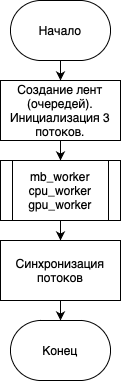
\includegraphics[scale=1]{main.png}
    \caption{Схема запуска конвейеров}
    \label{img:main}
\end{figure}

\begin{figure}[H]
    \centering
    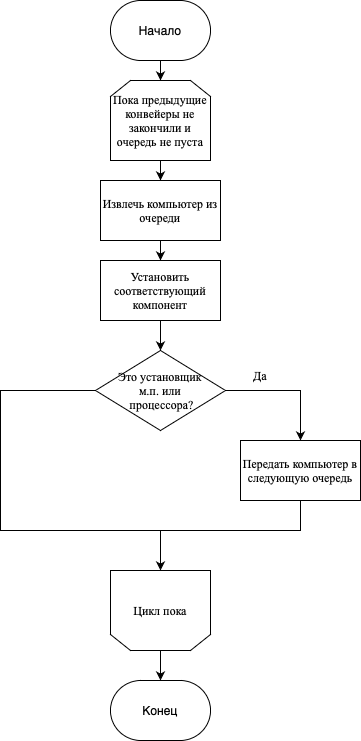
\includegraphics[scale=0.95]{worker.png}
    \caption{Схема работы одного конвейера}
    \label{img:worker}
\end{figure}

\subsection{Описание используемых типов данных}

При реализации алгоритмов будут использованы следующие структуры данных:

\begin{enumerate}
    \item Конвейер ~---~ очередь.
    \item Время установки компонента ~---~ целочисленный тип long long.
    \item Номер компьютера ~---~ целочисленный тип long long.
\end{enumerate}

\subsection{Структура программного обеспечения}

Программное обеспечение состоит из следующих модулей:

\begin{enumerate}
    \item main.cpp ~---~ модуль, содержащий код точки входа.
    \item queue.h  ~---~ модуль, содержащий код реализации очереди.
    \item dns.cpp  ~---~ модуль, содержащий код конвейера.
    \item computer.h ~---~ модуль, содержащий код класса компьютера.
\end{enumerate}

\subsection{Вывод}

В данном разделе были рассмотрены схемы алгоритма, описаны используемые типы данных, структура программного обеспечения.

\section{Технологическая часть}

В данном разделе приведены средства реализации и листинги кода.

\subsection{Средства реализации}

К языку программирования выдвигаются следующие требования:

\begin{enumerate}
    \item Возможность порождать системные потоки.
    \item Возможность производить замер времени выполнения части программы.
    \item Существуют среды разработки для этого языка.
\end{enumerate}

По этим требованиям был выбран язык программирования C++.

\subsection{Листинги кода}

\begin{lstlisting}[caption=Реализация очереди, label=list:queue, language={}]
#pragma once

#include <queue>
#include <mutex>
#include <condition_variable>

template <class T>
class SafeQueue
{
public:
    SafeQueue(void) : q(), m(), c() {}
    ~SafeQueue(void) {}

    bool empty() const {
        std::lock_guard<std::mutex> lock(m);
        return q.empty();
    }

    size_t size() const {
        std::lock_guard<std::mutex> lock(m);
        return q.size();
    }
    

    void enqueue(T t)
    {
        std::lock_guard<std::mutex> lock(m);
        q.push(t);
        c.notify_one();
    }

    T dequeue(void)
    {
        std::unique_lock<std::mutex> lock(m);
        while (q.empty()) {
            c.wait(lock);
        }

        T val = q.front();
        q.pop();
        return val;
    }
private:
    std::queue<T> q;
    mutable std::mutex m;
    std::condition_variable c;
};	
\end{lstlisting}

\begin{lstlisting}[caption=Класс компьютера, label=list:computer, language={}]
#pragma once

#include <chrono>
#include <thread>


class Computer {
public:
    Computer() = default;

    bool is_built() const { return mother_board && cpu && gpu; }
    
    bool mb_installed() const { return mother_board; }
    bool cpu_installed() const { return cpu; }
    bool gpu_installed() const { return gpu; }

    void set_id(size_t i) { id = i; }
    size_t get_id() const { return id; }

    void install_mb()  { std::this_thread::sleep_for(mb_installation_time);  mother_board = true; }
    void install_cpu() { std::this_thread::sleep_for(cpu_installation_time); cpu = true; }
    void install_gpu() { std::this_thread::sleep_for(gpu_installation_time); gpu = true; }


    long long mb_install_time_s;
    long long mb_install_time_e;
    long long cpu_install_time_s;
    long long cpu_install_time_e;
    long long gpu_install_time_s;
    long long gpu_install_time_e;

private:
    bool mother_board;
    bool cpu;
    bool gpu;

    size_t id;

    const std::chrono::microseconds mb_installation_time  {1500};
    const std::chrono::microseconds cpu_installation_time {1000};
    const std::chrono::microseconds gpu_installation_time {1100};
};
\end{lstlisting}

\begin{lstlisting}[caption=Работа конвейеров, label=list:conveyor, language={}]
void dns::run_parallel() {
    std::vector<Computer> comps(ncomps);

    for (size_t i = 1; i <= comps.size(); i++) {
        comps[i - 1].set_id(i);
    }

    SafeQueue<Computer*> mb_man;
    SafeQueue<Computer*> cpu_man;
    SafeQueue<Computer*> gpu_man;

    std::atomic_bool mb_done  = false;
    std::atomic_bool cpu_done = false;

    auto qs = std::chrono::high_resolution_clock::now();


    auto mb_worker = [qs, &mb_done, &m = mb_man, &c = cpu_man]() {
        while (!m.empty()) {
            auto comp = m.dequeue();
            auto s = std::chrono::high_resolution_clock::now();
            comp->install_mb();
            auto e = std::chrono::high_resolution_clock::now();

            comp->mb_install_time_s = std::chrono::duration_cast<std::chrono::microseconds>(s - qs).count();
            comp->mb_install_time_e = std::chrono::duration_cast<std::chrono::microseconds>(e - qs).count();

            c.enqueue(comp);
        }

        mb_done = true;   
    };

    auto cpu_worker = [qs, &cpu_done, &mb_done, &c = cpu_man, &g = gpu_man]() {
        while (1) {
            if (!c.empty()) {
                auto comp = c.dequeue();
                auto s = std::chrono::high_resolution_clock::now();
                comp->install_cpu();
                auto e = std::chrono::high_resolution_clock::now();

                comp->cpu_install_time_s = std::chrono::duration_cast<std::chrono::microseconds>(s - qs).count();
                comp->cpu_install_time_e = std::chrono::duration_cast<std::chrono::microseconds>(e - qs).count();

                g.enqueue(comp);
            } else if (mb_done) {
                break;
            }
        }

        cpu_done = true;
    };

    auto gpu_worker = [qs, &cpu_done, &mb_done, &g = gpu_man]() {
        while (1) {
            if (!g.empty()) {
                auto comp = g.dequeue();
                auto s = std::chrono::high_resolution_clock::now();
                comp->install_gpu();
                auto e = std::chrono::high_resolution_clock::now();

                comp->gpu_install_time_s = std::chrono::duration_cast<std::chrono::microseconds>(s - qs).count();
                comp->gpu_install_time_e = std::chrono::duration_cast<std::chrono::microseconds>(e - qs).count();
            } else if (cpu_done && mb_done){
                break;
            }
        }
    };


    for (auto &&c : comps) {
        mb_man.enqueue(&c);
    }

    qs = std::chrono::high_resolution_clock::now();

    auto mb_t  = std::thread(mb_worker);
    auto cpu_t = std::thread(cpu_worker);
    auto gpu_t = std::thread(gpu_worker);


    mb_t.join();
    cpu_t.join();
    gpu_t.join();

    auto qe = std::chrono::high_resolution_clock::now();

    std::cout << "End time: " << std::chrono::duration_cast<std::chrono::microseconds>(qe - qs).count() << "\n";

    print_comps(comps);
}
\end{lstlisting}

\subsection{Вывод}

В данном разделе был разработан конвейер.

\section {Исследовательский раздел}

В данном разделе будет проведен замер временных характеристик выполнения алгоритмов и пример работы программы.

\subsection{Пример работы программы}

\begin{figure}[H]
    \centering
    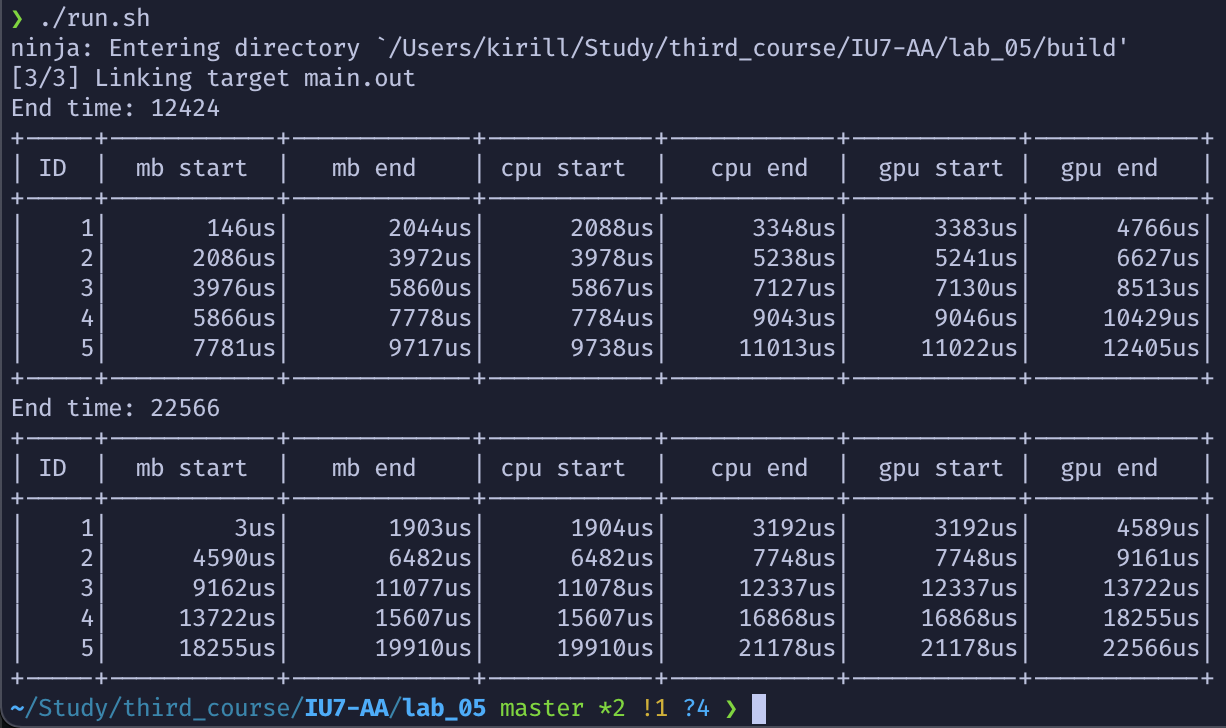
\includegraphics[scale=0.7]{ex_run.png}
    \caption{Пример работы программы}
    \label{img:example_run}
\end{figure}


\subsection{Технические характеристики}

Технические характеристики электронно-вычислительной машины, на которой выполнялось тестирование:

\begin{itemize}
    \item операционная система: macOS BigSur версия 11.4;
    \item оперативная память: 8 гигабайт LPDDR4;
    \item процессор: Apple M1.
\end{itemize}

\subsection{Время работы программы}

В таблице \ref{tab:time} представлен лог работы программы. Лента 1 занимается установкой материнской платы, лента 2 --- установкой центрального процессора, лента 3 --- установка графического процессора. Время указано в микросекундах. \\

\begin{table}[H]
    \caption{\centering Лог работы конвейерной обработки программы}
    \centering
    \begin{tabular}{|c|c|c|c|}
    \hline
    \multicolumn{1}{|l|}{Лента №} & \multicolumn{1}{l|}{Задача №} & \multicolumn{1}{l|}{Время начала} & \multicolumn{1}{l|}{Время конца} \\ \hline
    1                             & 1                             & 40                                & 1951                             \\ \hline
    2                             & 1                             & 1966                              & 3221                             \\ \hline
    3                             & 1                             & 3227                              & 4403                             \\ \hline
    1                             & 2                             & 1962                              & 3865                             \\ \hline
    2                             & 2                             & 3876                              & 5132                             \\ \hline
    3                             & 2                             & 5137                              & 6516                             \\ \hline
    1                             & 3                             & 3873                              & 5781                             \\ \hline
    2                             & 3                             & 5789                              & 7044                             \\ \hline
    3                             & 3                             & 7059                              & 8439                             \\ \hline
    1                             & 4                             & 5789                              & 7669                             \\ \hline
    2                             & 4                             & 7672                              & 8927                             \\ \hline
    3                             & 4                             & 8932                              & 10314                            \\ \hline
    1                             & 5                             & 7671                              & 9554                             \\ \hline
    2                             & 5                             & 9559                              & 10816                            \\ \hline
    3                             & 5                             & 10817                             & 12200                            \\ \hline
    \end{tabular}
    \label{tab:time}
\end{table}

На рисунке \ref{img:plot} представлен график зависимости времени работы реализации конвейеров от количества задач для линейной и параллельной обработки конвейера.

\begin{figure}[H]
    \centering
    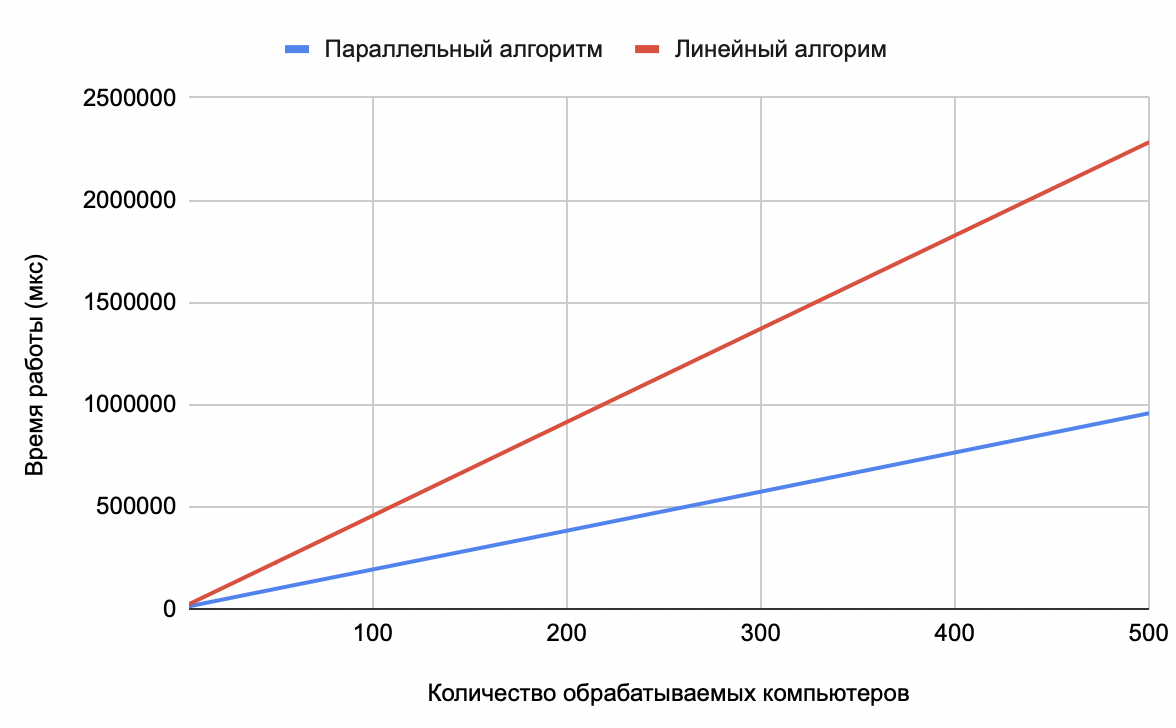
\includegraphics[scale=0.8]{plot.png}
    \caption{Зависимость времени работы реализации конвейеров от количества задач}
    \label{img:plot}
\end{figure}

\subsection{Вывод}

Параллельная реализация конвейерной обработки значительно выигрывает по времени относительно линейной реализации. Как видно из рисунка \ref{img:plot}, линейная реализация примерно в 2 раза медленнее параллельной при 500 задачах.


\anonsection{Заключение}

В результате выполнения лабораторной работы было экспериментально подтверждено различие временных характеристик последовательной и параллельной реализации конвейерной обработки данных.

В рамках выполнения работы была достигнута цель и решены следующие задачи:

\begin{enumerate}
	\item изучили освоили конвейерную обработку данных;
	\item применили изученные основы для реализации конвейерной обработки данных;
	\item получили практические навыки;
	\item получили статистику выполнения программы;
	\item описали и обосновали полученные результаты;
	\item выбрали и обосновали языка программирования, для решения данной задачи.
\end{enumerate}

\anonsection{Список литературы}

\begin{enumerate}
	\item Visual Studio Code [Электронный ресурс], режим доступа: https://code.visualstudio.com/ (дата обращения: \today)
	\item LPDDR4 [Электронный ресурс] \url{https://ru.wikipedia.org/wiki/LPDDR#LPDDR4} (дата обращения: \today)
	\item Ульянов М. В. Ресурсно-эффективные компьютерные алгоритмы. Разработка и Анализ. - Наука Физматлит, 2007. - 376.
	\item Библиотека Chrono [Электронный ресурс] Режим доступа: https://en. cppreference.com/w/cpp/chrono (дата обращения: \today).
	\item Библиотека для работы с потоками thread [Электронный ресурс] Режим доступа: https://en.cppreference.com/w/cpp/thread (дата обращения: \today).
\end{enumerate}

\end{document}

\end{document}
